\section{Simhash-based Website Model}
\label{s:methodology}



in order to detect cloaking, we design a much more efficient algorithm with
comparable false positive rate and true positive rate.

There are two challenges in cloaking detection: reveal the content and handle
dynamics of a webpage.
In order 

In order to detect cloaking,
Challenges and solutions. Basic ideas are 1, 2, 3.




\subsection{Simhash-based Website Model}
Methodology of dynamic modeling of web pages
\subsubsection{Distance Approximation}
Simhash~\cite{charikar2002similarity} is a hash function family that maps a high dimension dataset into fixed
bits and preserves the following attribute:

Suppose P and Q are probability distributions over L, 
\begin{multline}
  EMD(P, Q) \le E[d(h(P), h(Q))] \\
  \le O(\log{n}\log{\log{n}})EMD(P, Q).
\end{multline}

This equation is telling us that the hamming distance between simhash of set
\b{P} and set \b{Q} is an approximation of Earth Moving Distance(EMD) between set P
and Q. Charikar~\cite{charikar2002similarity} give the formal proof that the
hamming distance of sets represents the cosine similarity.
~\cite{manku2007detecting} implements an algorithm for creating text-based
simhash for a website. In our work, we use the same simhash algorithm,


\subsubsection{Insights On Feature Set Selection}



\subsubsection{Computation}


\subsubsection{Text Simhash and Dom Simhash}


In order to compress text information of a document, we extract the same set of
text features as ~\cite{manku2007detecting}.

Inspired from previous work, we understand that looking at only text would raise
high false positive, therefore, we take into consideration the tag.

In order to compress the structural 

for compressing
the text information. 



In order to detect cloaking, we need to capture the bahavior and similarity that
a same website maintains. That is to say, we not only need to look at the text-based simhash,
but also dom-based simhash. We implemented the text-simhash algorithm described
in ~\cite{manku2007detecting}, which extract words, bi-gram, tri-gram set
(repeated elements only recorded once) from a website and compute simhash using
simhash algorithm described in ~\cite{charikar2002similarity}.

There is no current algorithm for generating dom simhash. Therefore, we design
an algorithm to perform this task. For each dom tree, we record the node set, as
well as the child parent pair set. The node set tells us information about what
tag is present in this page, and child parent pair tells us how these tags are
organized.

% you can also use the wonderful epsfig package...
\begin{figure}[t]
  \centering
  \begin{subfigure}
    \centering
    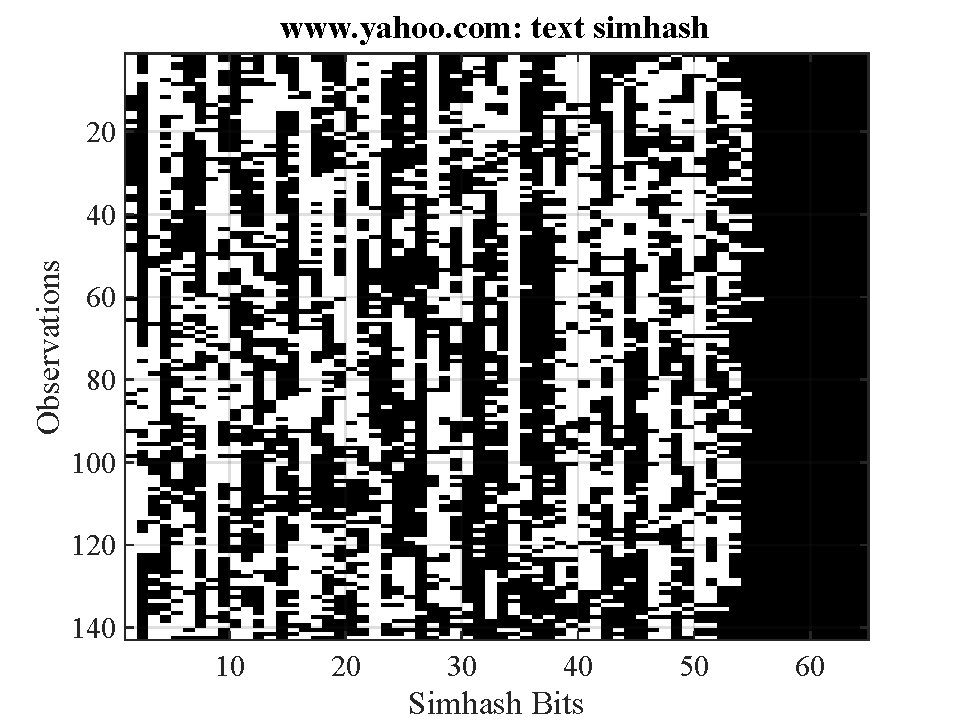
\includegraphics[width=.5\textwidth]{fig/yahoo-text-user}
    \label{fig:yahoo-text-user}
  \end{subfigure}%
  \begin{subfigure}
    \centering
    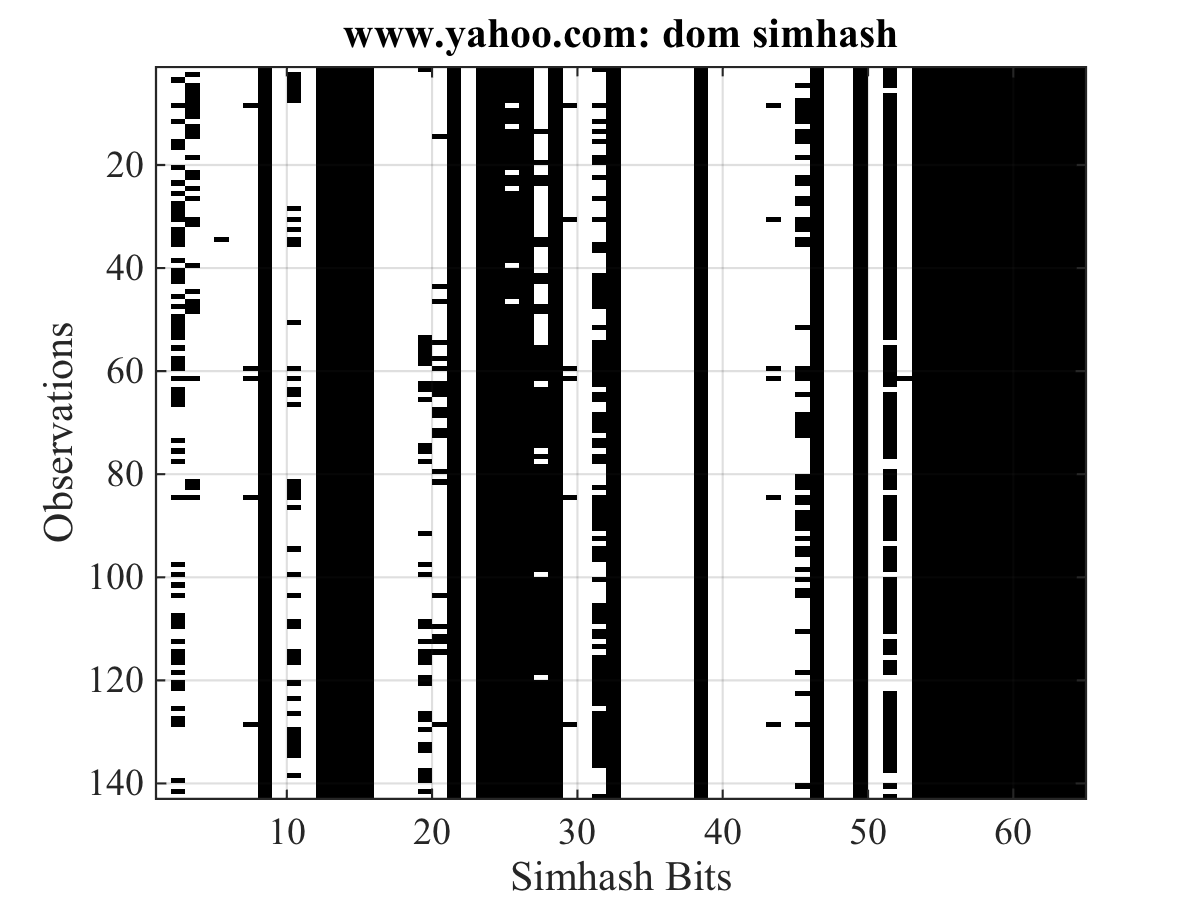
\includegraphics[width=.5\textwidth]{fig/yahoo-dom-user}
    \label{fig:yahoo-dom-user}
  \end{subfigure}
  \caption{Yahoo simhash changes over 7x24 period Feb.1 - 7, 2015}
  \label{fig:yahoo-simhash}
\end{figure}





It is pretty straightforward from ~\autoref{fig:yahoo-simhash} that,
text simhash changes rapidly, indicating dynamic nature of this
website, and dom simhash changes relatively slow and less.

Till now, we have demonstrated the algorithm we are using to generate
text-simhash and dom-simhash out of a website. Based on our observation, the
text-simhash may change rapidly, while dom-simhash relatively remain the same.


\subsubsection{Aggregating / Clustering}
Assume we are monitoring the same website over a period of time. This website
have dynamic changes all the time. But there can be another kind of change -
whole page change. In this case, it is reasonable to first separate them apart
and look at each of them.


Hamming distance is a special case of Euclidean distance. We can take the
average to represent the center of these points.


Using the hamming distance measure on a dimension of 64-bit.


For different websites, simhash can be considered as an algorithm to map them to
a 64-bit number randomly ~\cite{manku2007detecting}. For the same website,
simhash measures the similarity between them.



\begin{figure}[t]
  \centering
  \begin{subfigure}
    \centering
    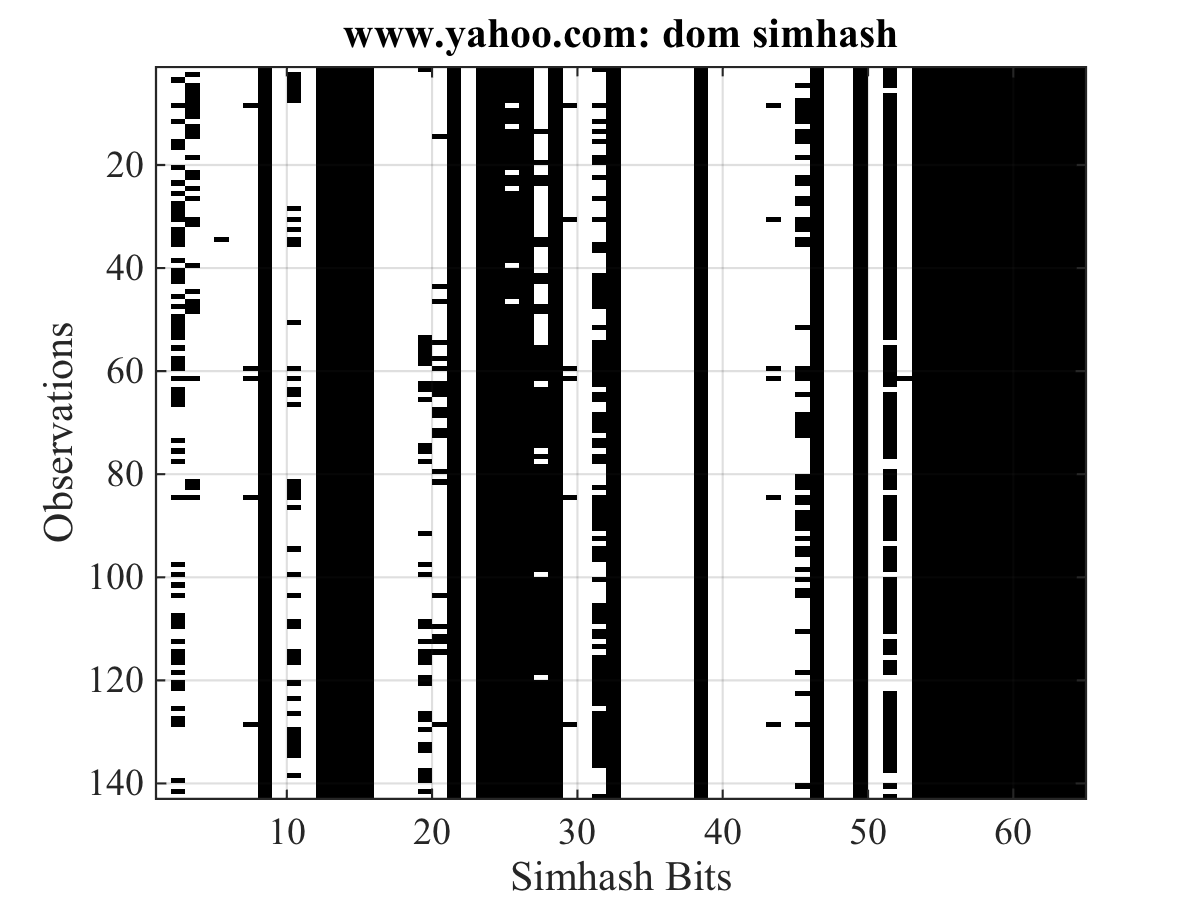
\includegraphics[width=.5\textwidth]{fig/yahoo-dom-user}
    \label{fig:yahoo-dom-user}
  \end{subfigure}%
  \begin{subfigure}
    \centering
    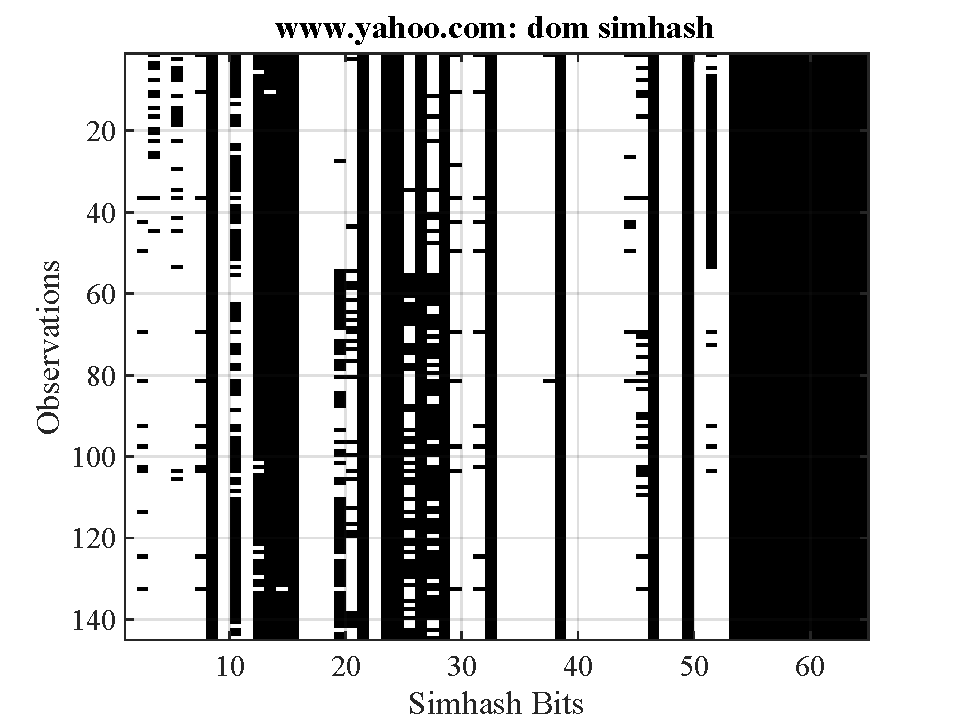
\includegraphics[width=.5\textwidth]{fig/yahoo-dom-google}
    \label{fig:yahoo-dom-google}
  \end{subfigure}
  \caption{Comparison of user and google seen dom simhash}
  \label{fig:yahoo-simhash}
\end{figure}




Different from ~\cite{manku2007detecting}, we not only want to know whether two pages are
duplicate, we also want to know the patterns of these simhash. In this work, we employ
hierarchical clustering to do this job.

In hierarchical clustering uses a set of dissimilarities for the n objects being clustered.
Initially, each object is assigned to its own cluster and then the algorithm
proceeds iteratively, the complete linkage method finds similar clusters.

In order to decide the number of clusters to take in hierarchical clustering
(when to stop), we use inconsistent coefficient.


L1 norm : sum of the differences in
each dimension

considerations of significance, we ask whether this is an unusual result or
whether it could have arisen merely by chance


The inconsistency coefficient characterizes each link in a cluster tree by
comparing its height with the average height of other links at the same level of
the hierarchy. The higher the value of this coefficient, the less similar the
objects connected by the link.

One way to determine the natural cluster divisions in a data set is to compare
the height of each link in a cluster tree with the heights of neighboring links
below it in the tree.

linkage metric: hammming
method: Unweighted average distance (UPGMA)
cutoff: inconsistent value less than c
pick inconsistent value now!!!!!

learning 1.1
detection 2.0


\begin{gather*} \label{npa}
  d(u,v) = \min(dist(u[i],v[j])) \\
  \text{for all points i in cluster u and j in
  cluster v. }
\end{gather*}
This~\autoref{npa} is known as the Nearest Point Algorithm.

Single-linkage clustering is one of several methods of agglomerative
hierarchical clustering. In the beginning of the process, each element is in a
cluster of its own. The clusters are then sequentially combined into larger
clusters, until all elements end up being in the same cluster. The stop
criterion is the distance one.


\subsection{Data collection and Groundtruth}

1. Collect terms
2. Query search results.
3. Crawl data and get ground truth (how
many).
4. Train model and select parameters use 5-fold stratified cross validation
~\cite{scikit-learn}.

\subsection{Cloaking Detection}



Classification hinges on having access to a robust set of features derived from
URLs to discern between spam and non-spam. Previous work has shown that lexical
properties of URLs, page content, and hosting properties of domains are all
effective routes for classification [15], [16], [22]–[24]. We expand upon these
ideas, adding our own sources of features collected by one of three components:
a web browser, a DNS resolver, and IP address analysis. A comprehensive list of
features and the component that collects them can be found in Table 1. A single
monitor oversees multiple copies of each component to aggregate results and
restart failed processes. In turn, the monitor and feature collection components
are bundled into a crawling instance and replicated in the cloud


%\subsection{Model Selection}
%
%
%\begin{table*}[!th]                                                     
%  \centering                                                            
%  \scriptsize                                                           
%  \begin{tabular}{lllllllllll}
  \toprule
  & \multicolumn{2}{c}{\textbf{Normal}}
  & \multicolumn{2}{c}{\textbf{Lognormal}}
  & \multicolumn{2}{c}{\textbf{Exponential}}
  & \multicolumn{2}{c}{\textbf{Gamma}}
  & \multicolumn{2}{c}{\textbf{Logistic}}\\

  \textbf{Website(Hash Type)\textbackslash Model}
  & AD-value
  & P-value
  & AD-value
  & P-value
  & AD-value
  & P-value
  & AD-value
  & P-value
  & AD-value
  & P-value \\
  \midrule
  digg.com T & 0.617 &  0.100 & 0.481 &  0.219 &
  14.851 & < 0.003 & 0.538 &  0.186 & 0.531 &  0.131\\ 
  digg.com T & 0.227 &  0.806 & 0.179 &  0.914 &
  19.690 &  < 0.003 & 0.198 &  > 0.250 & 0.250 & >0.250\\
  yahoo.com T & 0.192 &  0.893 & 0.263 &  0.692 &
  35.828 & <0.003 &   0.231 & >0.250 & 0.222 & >0.250\\
  amazon.com T & 0.720 &  0.058 & 0.323 &  0.520 & 
  27.754 & <0.003 &  0.436 & >0.250 & 0.642 &  0.058\\
  reddit.com T & 0.373 &  0.411 & 0.331  & 0.509 & 
  35.063 & <0.003 & 0.340 & >0.250 & 0.361 & >0.250\\
  yacombinator.com T & 0.473 &  0.237 & 0.516 &  0.186 &
  37.551 & <0.003 & 0.519 &  0.204 & 0.583 &  0.089\\

  digg.com D & 0.319 &  0.372 & 0.348 &  0.305 &
  1.491 &  0.021 &  0.402 & >0.250 & 0.363 & >0.250\\
  yahoo.com D & 0.531 &  0.168 & 0.392 &  0.366 &
  18.837 & <0.003 & 0.441 & >0.250 & 0.584  & 0.088\\
  amazon.com D & 1.519 & <0.005 & 0.916 &  0.019 &
  22.083 & <0.003 & 1.052 &  0.009 & 0.548 &  0.114\\
  amazon.com D & 0.483 & 0.117 &  0.504 & 0.104 &
  1.741 & 0.010 & 0.601 & 0.128 & 0.523 & 0.115\\

\end{tabular}

                                     
%  \caption{Model statistics for selected websites}
%  \label{tbl:para-select}                                         
%\end{table*}                                                            
%
%
%This table ~\autoref{tbl:para-select} shows the Anderson-Darling (AD) value and P-value for each model.
%A common rule used in model selection is pick the model which has the smallest
%value with P-value greater than 5\%. Each row in the table represents one
%website. From the statistics of these websites, we choose normal distribution
%for text simhash and Lognomal distribution for dom simhash.
%
%In the simhash based cloaking detection model, input from the user is simply simhash. How to compare against the simhashs that is already collected?
%
%One simple way is to compute the average distance from this simhash to all the observed simhashs. The next step is then to tell whether this distance is reasonable. 
%
%The text distribution follows lognormal distribution.
%After mannual check of those results.
%
%
%
%
%You have to run {\tt latex} once to prepare your references for
%munging.  Then run {\tt bibtex} to build your bibliography metadata.
%Then run {\tt latex} twice to ensure all references have been resolved.
%If your source file is called {\tt usenixTemplate.tex} and your {\tt
%bibtex} file is called {\tt usenixTemplate.bib}, here's what you do:
%{\tt \small
%  \begin{verbatim}
%  latex usenixTemplate
%  bibtex usenixTemplate
%  latex usenixTemplate
%  latex usenixTemplate
%  \end{verbatim}
%}
%

